
\documentclass[12pt]{beamer}
\usepackage{xcolor}
\usepackage{pgf,pgfarrows,pgfnodes,pgfautomata,pgfheaps,pgfshade}
\usetheme{Air}

\DeclareMathOperator*{\argmax}{arg\,max}

\title[CSC349A Numerical Analysis]{CSC349A Numerical Analysis}


\logo{\pgfputat{\pgfxy(-0.5,7.5)}{\pgfbox[center,base]{
\includegraphics[width=1.0cm]{figures/uvic}}}}  
\beamertemplatenavigationsymbolsempty

    \defbeamertemplate{footline}{author and page number}{%
      \usebeamercolor[fg]{page number in head/foot}%
      \usebeamerfont{page number in head/foot}%
      \hspace{1em}\insertshortauthor\hfill%
      \insertpagenumber\,/\,\insertpresentationendpage\kern1em\vskip2pt%
    }
    \setbeamertemplate{footline}[author and page number]{}



\subtitle[Lecture 9]{Lecture 9}
\date[2023]{2023}
\author[R. Little]{Rich Little}
\institute[University of Victoria]{University of Victoria}
%\logo{\includegraphics[scale=.25]{unilogo.pdf}}
\begin{document}
\frame{\maketitle} % <-- generate frame with title


\AtBeginSection[]
{
\begin{frame}<beamer>[allowframebreaks]{Table of Contents}
\tableofcontents[currentsection,currentsubsection, 
    hideothersubsections, 
    sectionstyle=show/shaded,
]
\end{frame}
}






\section{Newton-Raphson} 

\begin{frame}{Geometric derivation}
\begin{itemize}
\item{The real roots of a function $f(x)$ occur when the graph of the
function intersects with the x-axis.} 
\item{The main idea behind the
Newton/Raphson method for root finding is given an initial
approximation $x_0$ to a zero of $f(x)$ to approximate the graph of f(x)
at $x_0$ by the tangent line - essentially linearizing the function in
that area.}
\end{itemize}

\end{frame}

\begin{frame}{An illustrative example} 

\begin{figure}[hbt!]
  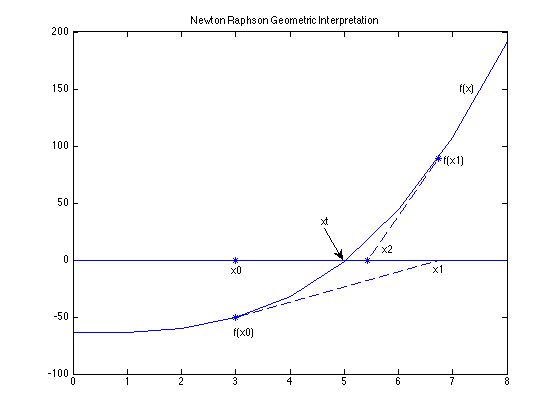
\includegraphics[scale=0.45]{newton}
%   \caption{Geometric interpetation of the Newton Raphson method}
  \label{fig:newton}
\end{figure}
\end{frame}  

\begin{frame}{Newton-Raphson Formula}

Each iteration we approximate the root $x_t$ with $x_{i+1}$ based on previous approximation $x_i$ using,
\begin{equation}
x_{i+1}=x_i - \frac{f(x_i)}{f'(x_i)}
\end{equation}

\noindent
with the hope that 

\begin{equation}
\lim_{i \rightarrow \infty} x_i = x_t 
\end{equation} 
\end{frame}

\begin{frame}{Example 1} 

Estimate the root of $f(x) = e^{-x} -x$ employing an initial guess of
$x_0 = 0$. Note that the true root is $x_t=0.56714329$.
\vspace{3 in}
\end{frame}

\begin{frame}{Example 1 continued} 

Estimate the root of $f(x) = e^{-x} -x$ employing an initial guess of
$x_0 = 0$. The iterative equation can be applied to compute: 

\begin{table}[h]
\begin{tabular}{c|c|c} 
$i$ & $x_i$ & $\varepsilon_t(\%)$ \\ 
\hline 
$0$ & $0$ & $100$ \\
$1$ & $0.5$ & $11.8$ \\ 
$2$ & $0.566311003$ & $0.147$ \\
$3$ & $0.567143165$ & $0.0000220$ \\ 
$4$ & $0.567143290$ & $<10^{-8}$ \\  
\hline
\end{tabular} 
\end{table} 
\noindent 
Notice that the approach rapidly converges on the true root much faster than 
it would using {\it Bisection}. 
\end{frame} 

\section{Newton method convergence}

\begin{frame}{Derivation using Taylor's theorem}

Recall the Taylor theorem for $f(x)$ with $n=1$ expanded about $a=x_i$:

\begin{equation} 
f(x) = f(x_i) + f'(x_i)(x-x_i) + \frac{f''(\xi)}{2}(x-x_i)^2
\end{equation}
\noindent 
for some value $\xi$ between $x$ and $x_i$.
\end{frame} 

\begin{frame}{Convergence} 

  The derivation of the Newton/Raphson method gives insight into how
fast Newton's method converges:
\\
First we evaluate the Taylor Theorem at $x=x_t$, an exact zero: 

\begin{equation} 
0 = f(x_t) = f(x_i) + (x_t-x_i)f'(x_i) + \frac{(x_t-x_i)^2}{2}f''(\xi)
\end{equation} 

Newton's method $x_{i+1} = x_{i} - \frac{f(x_i)}{f'(x_i)}$ can be rewritten as: 
\begin{equation} 
0 = f(x_i) + (x_{i+1} -x_{i}) f'(x_{i})
\end{equation} 
\vspace{1 in}
\end{frame} 

\begin{frame}{Convergence II} 

If we subtract the last two equations (4,5) then we get: 

\begin{equation} 
0 = (x_t -x_{i+1}) f'(x_i) + \frac{(x_t - x_i)^2}{2}f''(\xi)
\end{equation} 
\noindent and if we let $E_{i+1} = x_t - x_{i+1}$ and $E_i = x_t - x_{i}$ denote the error in $x_{i+1}, x_i$ then we have: 
\[
0 = E_{i+1} f'(x_i) + \frac{E_i^2}{2} f''(\xi) \;\;\; \mbox{thus} \;\;
\frac{E_{i+1}}{E_i^2} = \frac{-f''(\xi)}{2f'(x_{i})} 
\]

\end{frame} 


\begin{frame}{Order of convergence}
{\bf Definition} (not in textbook) \\ 
If a sequence ${x_0, x_1, x_2, x_3, \dots }$ converges to $x_t$ that is 
$\lim_{i \rightarrow \infty}x_i = x_t$ and $E_i = x_t - x_i$, then the order of converge of the sequence is $\alpha$ if there are constants $\lambda > 0$ and $\alpha \geq 1$ such that: 
\begin{equation} 
\lim_{i \rightarrow \infty} \frac{|E_{i+1}|}{|E_i|^{\alpha}} = \lambda 
\end{equation} 
\end{frame} 


\begin{frame} 
In general, $\lambda$ and $\alpha$ depend on the algorithm used to compute ${x_i}$, on $f(x)$, and on the multiplicity of the zero $x_t$. 


{\bf Most common case:} 
\\ 
$\alpha = 1$ linear convergence \\ 
For large $i$, $|E_{i+1}| \approx \lambda |E_i|$ \\ 


In this case, successive errors decrease approximately by a constant amount: 
\begin{eqnarray*} 
|E_{i+1}| &\approx & \lambda |E_i| \\ 
|E_{i+2}| &\approx &  \lambda |E_{i+1}| \approx \lambda^2 |E_i|\\ 
|E_{i+3}| & \approx &  \lambda |E_{i+2}| \approx \lambda^3 |E_i|\\ 
\mbox{etc} \\ 
\end{eqnarray*} 

Errors $|E_{i+1}| \rightarrow 0$, that is $\lim_{i \rightarrow \infty}
x_i = x_t$ only if $0 < \lambda < 1$.
\end{frame} 

\begin{frame}{Quadratic convergence} 
For $\alpha = 2$ we have quadratic convergence. For large $i$, $|E_{i+1}| \approx \lambda |E_i|^2$ 
\\
After some error $|E_i| < 1$, convergence is rapid as the number of correct significant digits approximately doubles with each iteration e.g if 
$|E_i| = 10^{-t}$, then $|E_{i+1}| \approx \lambda 10^{-2t}$. 
\end{frame} 

\begin{frame}{Convergence of Newton's method} 
For Newton's method above: 
\[ 
\frac{E_{i+1}}{E_{i}^2} = \frac{-f''(\xi)}{2f'(x_i)} 
\] 
\noindent for some $\xi$ between $x_i$ and $x_{i+1}$. 

\[
\lim_{i \rightarrow \infty} \frac{|E_{i+1}|}{|E_i|^2} = \lim_{i \rightarrow \infty} 
\frac{|f''(\xi)|}{2|f'(x_i)|} = \frac{|f''(x_t)|}{2|f'(x_t)|}
\]
\noindent 
which is a constant $\lambda$ provided that $f'(x_t) \neq 0$. 
\\
{\bf Result:} Newton's method converges quadratically to a zero $x_t$ provided that $f'(x_t) \neq 0$
\end{frame} 


\begin{frame}{Implementation}

\begin{tabbing}
  xxx \= xxx \= xxx \= xxx \kill
\> \textbf{function} root = Newton( $x_0$, $\varepsilon$, \texttt{imax},  $f(x)$, $f'(x)$ ) \\
\> $i \leftarrow 1$ \\
\> output heading \\
\> \textbf{while} $i \le $ \texttt{imax} \\
\> \> $root \leftarrow x_0 - f(x_0)/f'(x_0)$ \\
\> \> output $i$, root \\
\> \> \textbf{if} $|1-x_0/root| < \varepsilon$ \\
\> \> \> exit \\
\> \> \textbf{end if} \\
\> \> $i \leftarrow i + 1$ \\
\> \> $x_0 \leftarrow root$ \\
\> \textbf{end while} \\
\> output ``failed to converge"
\end{tabbing}
\end{frame} 

\begin{frame}{Implementation Note}
Note that in general, using $|f(root)| < \varepsilon$ is not a suitable
test for convergence (instead of testing approximation error). The
reason is that $|f(root)| < \varepsilon$ does not imply that the value
{\it root} is within distance of $\varepsilon$ of an exact root $x_t$. 
\end{frame}



\begin{frame}{Newton Convergence} 

{\bf Theorem}: If Newton's method is applied to $f(x) = 0$ producing 
a sequence $x_i$ that converges to a root $x_t$, and if $f'(x_t) \neq 0$, then 
then order of convergence is $2$. 
\begin{itemize}
\item{If $f'(x_t) = 0$ and Newton's method convergences to a root $x_t$, then we will see later that the order of convergence is NOT quadratic.}
\end{itemize} 

\end{frame} 

\begin{frame}{Example 1} 
An illustration of the quadratic convergence of Newton's method. Here $f(x) = cos(x) -x$. This was computed in MATLAB, so at most 16 correct digits are possible. The bold digits are all correct. 


\begin{table}[h] 
\begin{tabular}{c|l|c}
$i$ & $x_i$ & no. of correct digits \\ 
\hline
0   & $\frac{\pi}{4} = 0.{\bf 7}85398$ & 1 \\ 
1   & 0.{\bf 739}5361 & 3 \\ 
2   & 0.{\bf 7390851}78 & 7 \\ 
3   & 0.{\bf 73908513321516}10 & 14 \\ 
4   & 0.{\bf 7390851332151606}  & 16 \\ 
\end{tabular} 
\end{table} 

\end{frame} 

\begin{frame}{Example 2 (Newton)} 
Root of $x^3 + 4 x^2 -10 = 0$ with $p_0 = -100$. 

\begin{table}[h]
\begin{tabular}{l|c}
$p_0 = -100$ &  \\ 
$p_1 = -67.12$ &  \\ 
$p_2 = -45.21$ &  \\ 
$\dots$ & $\dots$ \\ 
$p_{14} = -2.54$ &  \\ 
$p_{15} = -3.14$ &  \\ 
$p_{16} = -2.80$ &  \\ 
$\dots$ & $\dots$ \\ 
$p_{21} = 1.9405$ &  no. of correct digits \\ 
$p_{22} = {\bf 1}.4793$ &  $1$ \\ 
$p_{23} = {\bf 1.3}711$ &  $2$ \\ 
$p_{24} = {\bf 1.365}25$ &  $4$ \\ 
$p_{25} = {\bf 1.365230001}1$  &  $9$ \\ 
\end{tabular} 
\end{table} 
\end{frame} 

\begin{frame}{Four Cases of Poor Convergence}
\begin{figure}[ht]
  \centering
  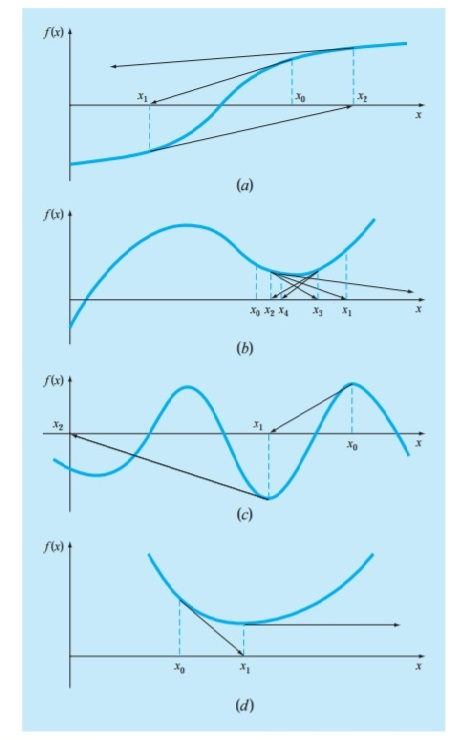
\includegraphics[scale=0.6]{BadNewton}
%   \caption{Geometric interpetation of the Newton Raphson method}
  \label{fig:BadNewton}
\end{figure}


\end{frame}

\begin{frame}{Newton Convergence} 

\begin{block}{Theorem} Suppose that $f(x),f'(x)$ and $f''(x)$ all exist and are continuous on some interval $[a,b]$, that $x_t \in [a,b]$ is a root of $f(x) = 0$, and that $f'(x_t) \neq 0$. Then there exists a value $\delta > 0$, such that Newton's method converges for all initial approximations $x_0 \in [x_t - \delta, x_t + \delta]$. 
\end{block} 
\end{frame} 

\begin{frame}{Note} 
In general there is no way to determine such a value $\delta$. This theorem only says that for all such functions $f(x)$, such a value $\delta$ exists. Even if the value of $\delta$ is extremely small, there is an interval of values around the root $x_t$ such that if $x_0$ (the initial approximation) lies in this interval, then Newton's method will converge. 

Thus the interpretation of the above theorem is that Newton's method always converges if the initial approximation $x_0$ is sufficiently close to the root $x_t$. 
\end{frame} 








\end{document}


